\iffalse
This file is protected by Copyright. Please refer to the COPYRIGHT file
distributed with this source distribution.

This file is part of OpenCPI <http://www.opencpi.org>

OpenCPI is free software: you can redistribute it and/or modify it under the
terms of the GNU Lesser General Public License as published by the Free Software
Foundation, either version 3 of the License, or (at your option) any later
version.

OpenCPI is distributed in the hope that it will be useful, but WITHOUT ANY
WARRANTY; without even the implied warranty of MERCHANTABILITY or FITNESS FOR A
PARTICULAR PURPOSE. See the GNU Lesser General Public License for more details.

You should have received a copy of the GNU Lesser General Public License along
with this program. If not, see <http://www.gnu.org/licenses/>.
\fi

%----------------------------------------------------------------------------------------
% Required document specific properties
%----------------------------------------------------------------------------------------
\def\docTitle{ZedBoard Getting Started Guide}
\def\snippetpath{../../../../../../doc/av/tex/snippets}
%----------------------------------------------------------------------------------------
% Global latex header (this must be after document specific properties)
%----------------------------------------------------------------------------------------
\iffalse
This file is protected by Copyright. Please refer to the COPYRIGHT file
distributed with this source distribution.

This file is part of OpenCPI <http://www.opencpi.org>

OpenCPI is free software: you can redistribute it and/or modify it under the
terms of the GNU Lesser General Public License as published by the Free Software
Foundation, either version 3 of the License, or (at your option) any later
version.

OpenCPI is distributed in the hope that it will be useful, but WITHOUT ANY
WARRANTY; without even the implied warranty of MERCHANTABILITY or FITNESS FOR A
PARTICULAR PURPOSE. See the GNU Lesser General Public License for more details.

You should have received a copy of the GNU Lesser General Public License along
with this program. If not, see <http://www.gnu.org/licenses/>.
\fi

% Sets OpenCPI Version used throughout all the docs. This is updated by
% scripts/update-release.sh when a release is being made and must not
% be changed manually.
\def\ocpiversion{v2.2.0}

\documentclass{article}
\author{}  % Force author to be blank
\date{OpenCPI Release:\ \ \ocpiversion}  % Force date to be blank and override date with version
\title{OpenCPI\\\docTitle}  % docTitle must be defined before including this file
%----------------------------------------------------------------------------------------
% Paper size, orientation and margins
%----------------------------------------------------------------------------------------
\usepackage{geometry}
\geometry{
  letterpaper,  % paper type
  portrait,     % text direction
  left=.75in,   % left margin
  top=.75in,    % top margin
  right=.75in,  % right margin
  bottom=.75in  % bottom margin
}
%----------------------------------------------------------------------------------------
% Header/Footer
%----------------------------------------------------------------------------------------
\usepackage{fancyhdr} \pagestyle{fancy}  % required for fancy headers
\renewcommand{\headrulewidth}{0.5pt}
\renewcommand{\footrulewidth}{0.5pt}
\lhead{\small{\docTitle}}
\rhead{\small{OpenCPI}}
%----------------------------------------------------------------------------------------
% Various packages
%----------------------------------------------------------------------------------------
\usepackage{amsmath}
\usepackage[page,toc]{appendix}  % for appendix stuff
\usepackage{enumitem}
\usepackage{graphicx}   % for including pictures by file
\usepackage{hyperref}   % for linking urls and lists
\usepackage{listings}   % for coding language styles
\usepackage{pdflscape}  % for landscape view
\usepackage{pifont}     % for sideways table
\usepackage{ragged2e}   % for justify
\usepackage{rotating}   % for sideways table
\usepackage{scrextend}
\usepackage{setspace}
\usepackage{subfig}
\usepackage{textcomp}
\usepackage[dvipsnames,usenames]{xcolor}  % for color names see https://en.wikibooks.org/wiki/LaTeX/Colors
\usepackage{xstring}
\uchyph=0  % Never hyphenate acronyms like RCC
\renewcommand\_{\textunderscore\allowbreak}  % Allow words to break/newline on underscores
%----------------------------------------------------------------------------------------
% Table packages
%----------------------------------------------------------------------------------------
\usepackage[tableposition=top]{caption}
\usepackage{float}
\floatstyle{plaintop}
\usepackage{longtable}  % for long possibly multi-page tables
\usepackage{multicol}   % for more advanced table layout
\usepackage{multirow}   % for more advanced table layout
\usepackage{tabularx}   % c=center,l=left,r=right,X=fill
% These define tabularx columns "C" and "R" to match "X" but center/right aligned
\newcolumntype{C}{>{\centering\arraybackslash}X}
\newcolumntype{M}[1]{>{\centering\arraybackslash}m{#1}}
\newcolumntype{P}[1]{>{\centering\arraybackslash}p{#1}}
\newcolumntype{R}{>{\raggedleft\arraybackslash}X}
%----------------------------------------------------------------------------------------
% Block Diagram / FSM Drawings
%----------------------------------------------------------------------------------------
\usepackage{tikz}
\usetikzlibrary{arrows,decorations.markings,fit,positioning,shapes}
\usetikzlibrary{automata}  % used for the fsm
\usetikzlibrary{calc}      % for duplicating clients
\usepgfmodule{oo}          % to define a client box
%----------------------------------------------------------------------------------------
% Colors Used
%----------------------------------------------------------------------------------------
\usepackage{colortbl}
\definecolor{blue}{rgb}{.7,.8,.9}
\definecolor{ceruleanblue}{rgb}{0.16, 0.32, 0.75}
\definecolor{cyan}{rgb}{0.0,0.6,0.6}
\definecolor{darkgreen}{rgb}{0,0.6,0}
\definecolor{deepmagenta}{rgb}{0.8, 0.0, 0.8}
\definecolor{maroon}{rgb}{0.5,0,0}
%----------------------------------------------------------------------------------------
% Define where to hyphenate
%----------------------------------------------------------------------------------------
\hyphenation{Cent-OS}
\hyphenation{install-ation}
%----------------------------------------------------------------------------------------
% Define Commands & Rename Commands
%----------------------------------------------------------------------------------------
\newcommand{\code}[1]{\texttt{#1}}  % For inline code snippet or command line
\newcommand{\sref}[1]{Section~\ref{#1}}  % To quickly reference a section
\newcommand{\todo}[1]{\textcolor{red}{TODO: #1}\PackageWarning{TODO:}{#1}}  % To do notes
\renewcommand{\contentsname}{Table of Contents}
\renewcommand{\listfigurename}{List of Figures}
\renewcommand{\listtablename}{List of Tables}

% This gives a link to gitlab.io document. By default, it outputs the filename.
% You can optionally change the link, e.g.
% \githubio{FPGA\_Vendor\_Tools\_Installation\_Guide.pdf} vs.
% \githubio[\textit{FPGA Vendor Tools Installation Guide}]{FPGA\_Vendor\_Tools\_Installation\_Guide.pdf}
% or if you want the raw ugly URL to come out, \githubioURL{FPGA_Vendor_Tools_Installation_Guide.pdf}
\newcommand{\githubio}[2][]{% The default is for FIRST param!
\href{http://opencpi.gitlab.io/releases/\ocpiversion/docs/#2}{\ifthenelse{\equal{#1}{}}{\texttt{#2}}{#1}}}
\newcommand{\gitlabcom}[2][]{% The default is for FIRST param!
\href{http://gitlab.com/opencpi/#2}{\ifthenelse{\equal{#1}{}}{\texttt{#2}}{#1}}}
\newcommand{\githubioURL}[1]{\url{http://opencpi.gitlab.io/releases/\ocpiversion/docs/#1}}
% Lastly, if you want a SINGLE leading path stripped, e.g. assets/X.pdf => X.pdf:
\newcommand{\githubioFlat}[1]{%
\StrBehind{#1}{/}[\den]%
\href{http://opencpi.gitlab.io/releases/\ocpiversion/docs/#1}{\texttt{\den}}%
}
%----------------------------------------------------------------------------------------
% VHDL Coding Language Style
% modified from: http://latex-community.org/forum/viewtopic.php?f=44&t=22076
%----------------------------------------------------------------------------------------
\lstdefinelanguage{VHDL}
{
  basicstyle=\ttfamily\footnotesize,
  columns=fullflexible,keepspaces,  % https://tex.stackexchange.com/a/46695/87531
  keywordstyle=\color{ceruleanblue},
  commentstyle=\color{darkgreen},
  morekeywords={
    library, use, all, entity, is, port, in, out, end, architecture, of,
    begin, and, signal, when, if, else, process, end,
  },
  morecomment=[l]--
}
%----------------------------------------------------------------------------------------
% XML Coding Language Style
% modified from http://tex.stackexchange.com/questions/10255/xml-syntax-highlighting
%----------------------------------------------------------------------------------------
\lstdefinelanguage{XML}
{
  basicstyle=\ttfamily\footnotesize,
  columns=fullflexible,keepspaces,
  morestring=[s]{"}{"},
  morecomment=[s]{!--}{--},
  commentstyle=\color{darkgreen},
  moredelim=[s][\color{black}]{>}{<},
  moredelim=[s][\color{cyan}]{\ }{=},
  stringstyle=\color{maroon},
  identifierstyle=\color{ceruleanblue}
}
%----------------------------------------------------------------------------------------
% DIFF Coding Language Style
% modified from http://tex.stackexchange.com/questions/50176/highlighting-a-diff-file
%----------------------------------------------------------------------------------------
\lstdefinelanguage{diff}
{
  basicstyle=\ttfamily\footnotesize,
  columns=fullflexible,keepspaces,
  breaklines=true,                            % wrap text
  morecomment=[f][\color{ceruleanblue}]{@@},  % group identifier
  morecomment=[f][\color{red}]-,              % deleted lines
  morecomment=[f][\color{darkgreen}]+,        % added lines
  morecomment=[f][\color{deepmagenta}]{---},  % Diff header lines (must appear after +,-)
  morecomment=[f][\color{deepmagenta}]{+++},
}
%----------------------------------------------------------------------------------------
% Python Coding Language Style
%----------------------------------------------------------------------------------------
\lstdefinelanguage{python}
{
  basicstyle=\ttfamily\footnotesize,
  columns=fullflexible,keepspaces,
  keywordstyle=\color{ceruleanblue},
  commentstyle=\color{darkgreen},
  stringstyle=\color{orange},
  morekeywords={
    print, if, sys, len, from, import, as, open,close, def, main, for, else,
    write, read, range,
  },
  comment=[l]{\#}
}
%----------------------------------------------------------------------------------------
% Fontsize Notes in order from smallest to largest
%----------------------------------------------------------------------------------------
%    \tiny
%    \scriptsize
%    \footnotesize
%    \small
%    \normalsize
%    \large
%    \Large
%    \LARGE
%    \huge
%    \Huge

\graphicspath{{figures/}}
%----------------------------------------------------------------------------------------

\begin{document}
\maketitle
\thispagestyle{empty}
\newpage

\begin{center}
	\textit{\textbf{Revision History}}
	\begin{table}[H]
		\label{table:revisions} % Add "[H]" to force placement of table
		\begin{tabularx}{\textwidth}{|c|X|l|}
			\hline
			\rowcolor{blue}
			\textbf{Revision} & \textbf{Description of Change} & \textbf{Date} \\
			\hline
			v1.1 & Initial Release & 3/2017 \\
			\hline
			v1.2 & Updated for OpenCPI Release 1.2 & 8/2017 \\
			\hline
			v1.3 & Updated for OpenCPI Release 1.3 & 2/2018 \\
			\hline
			pre-v1.4 & Fixed inaccurate description for hardware jumper configuration, OpenCPI-SD-zed directory path, and MAC address modification instructions for multiple ZedBoards on the same network. & 4/2018 \\
			\hline
			v1.4 & Update descriptions and paths & 9/2018 \\
			\hline
			v1.5 & Deprecated Zipper & 4/2019 \\
			\hline
			v1.6 & Refer to installation doc when possible & 1/2020 \\
	        \hline
		\end{tabularx}
	\end{table}
\end{center}
\newpage

\tableofcontents
\newpage

\section{References}
The reference(s) in Table 1 can be used as an overview of OpenCPI and may prove useful.  The installation guide is required since many of the steps mentioned here are defined there, especially in the section:  Enabling OpenCPI Development for Embedded Systems.  This document provides details for this system that can be applied to procedures defined there.  It is best to use both documents at the same time.  This document assumes a basic understanding of the Linux command line (or ``shell'') environment.  
\def\refcapbottom{}
\iffalse
This file is protected by Copyright. Please refer to the COPYRIGHT file
distributed with this source distribution.

This file is part of OpenCPI <http://www.opencpi.org>

OpenCPI is free software: you can redistribute it and/or modify it under the
terms of the GNU Lesser General Public License as published by the Free Software
Foundation, either version 3 of the License, or (at your option) any later
version.

OpenCPI is distributed in the hope that it will be useful, but WITHOUT ANY
WARRANTY; without even the implied warranty of MERCHANTABILITY or FITNESS FOR A
PARTICULAR PURPOSE. See the GNU Lesser General Public License for more details.

You should have received a copy of the GNU Lesser General Public License along
with this program. If not, see <http://www.gnu.org/licenses/>.
\fi

% This snippet creates the "References" table labeled "table:references"
% It creates three columns: Name, Publisher, Link and then inserts default documents
%
% To skip these defaults, define macros named
% refskipgs to skip "Getting Started"
% refskipig to skip "Installation Guide"
% refskipac to skip "Acronyms and Definitions"
% refskipocpiov to skip "OpenCPI Overview"
%
% See RPM_Installation_Guide.tex for examples
%
% After the defaults, it optionally inserts the "myreferences" macro that
% you defined elsewhere (you put hlines above all lines)
%
% If you want the \caption on the bottom, define "refcapbottom"
\begin{center}
\renewcommand*\footnoterule{} % Remove separator line from footnote
\renewcommand{\thempfootnote}{\arabic{mpfootnote}} % Use Arabic numbers (or can't reuse)
\begin{minipage}{0.9\textwidth}
  \begin{table}[H]
\ifx\refcapbottom\undefined
  \caption {References}
  \label{table:references}
\fi
  \begin{tabularx}{\textwidth}{|C|C|}
    \hline
    \rowcolor{blue}
    \textbf{Title} & \textbf{Link} \\
\ifx\refskipocpiov\undefined
    \hline
    OpenCPI User Guide & \githubio{OpenCPI\_User.pdf} \\
\fi
\ifx\refskipac\undefined
    \hline
    Acronyms and Definitions & \githubio{Acronyms\_and\_Definitions.pdf} \\
\fi
\ifx\refskipig\undefined
    \hline
    OpenCPI Installation Guide & \githubio{OpenCPI\_Installation.pdf} \\
\fi
\ifx\myreferences\undefined
\else
    \myreferences
\fi
    \hline
  \end{tabularx}
\ifx\refcapbottom\undefined
\else
  \caption {References}
  \label{table:references}
\fi
  \end{table}
\end{minipage}
\end{center}

\section{Overview}
This document provides: steps for configuring a factory provided Digilent Zedboard with the OpenCPI run-time environment for executing applications.

\section{Prerequisites}
\begin{flushleft}
It is assumed that the tasks defined in the ``Enabling OpenCPI Development for Embedded Systems'' section of the \githubio[\textit{OpenCPI Installation Guide}]{OpenCPI\_Installation\_Guide.pdf} have been successfully performed.
As mentioned there, support for the ZedBoard system is based on the \textit{ocpi.assets} built-in project, using the \textit{zed} OpenCPI HDL (FPGA) platform and the \textit{xilinx13\_4} or \textit{xilinx13\_3 }OpenCPI RCC (software) platform.  The software platforms are supported by the \textit{ocpi.core} built-in project.

\subsection{RCC Platforms}
The RCC platforms \textit{xilinx13\_3} and \textit{xilinx13\_4} are both supported. When targeting \textit{xilinx13\_4}, replace 13\_3 in directory names and other places where 13\_3 is used or applicable. Systems such as the E310 and ZedBoard use the same \textit{xilinx13\_4} RCC platform. If it is already installed and built it can apply to the ZedBoard. 

\subsection{Vendor Software Setup}
Also indicated in the installation guide, the tools used for software cross compilation are from the Xilinx Vivado 2013.4 SDK, and the tools used for the FPGA are any recent version of the Xilinx Vivado Webpack tools.  The Linux Kernel is based on the Xilinx Linux kernel tagged \textit{xilinx-v2013.4} (for \textit{xilinx13\_4}) or \textit{xilinx-v14.7} (for \textit{xilinx13\_3}.  The installation of these tools is described in the installation guide.

\subsection{Building Required Projects}
\label{sec:Building OpenCPI projects}
The standard built-in OpenCPI projects are built using the instructions in the installation guide.  This results in a single executable FPGA test application ready to run:  \textit{bias}, based on the \textit{testbias} HDL assembly, both in the \textit{assets} built-in project.

\subsection{Hardware Setup}
\begin{itemize}
\item \textbf{Digilent Zedboard Product Package}\\ \medskip
It is expected that this system includes a power supply, micro-USB to USB cable, micro-USB to female-USB adapter and standard SD card (4GB). \\ \medskip
OpenCPI has been tested on revisions C and D of the Zedboard.\\ \medskip
The micro-USB serial port located on the top-side of the ZedBoard labeled UART, can be used to access the serial connection with the processor.\medskip

\begin{figure}[H]
	\centerline{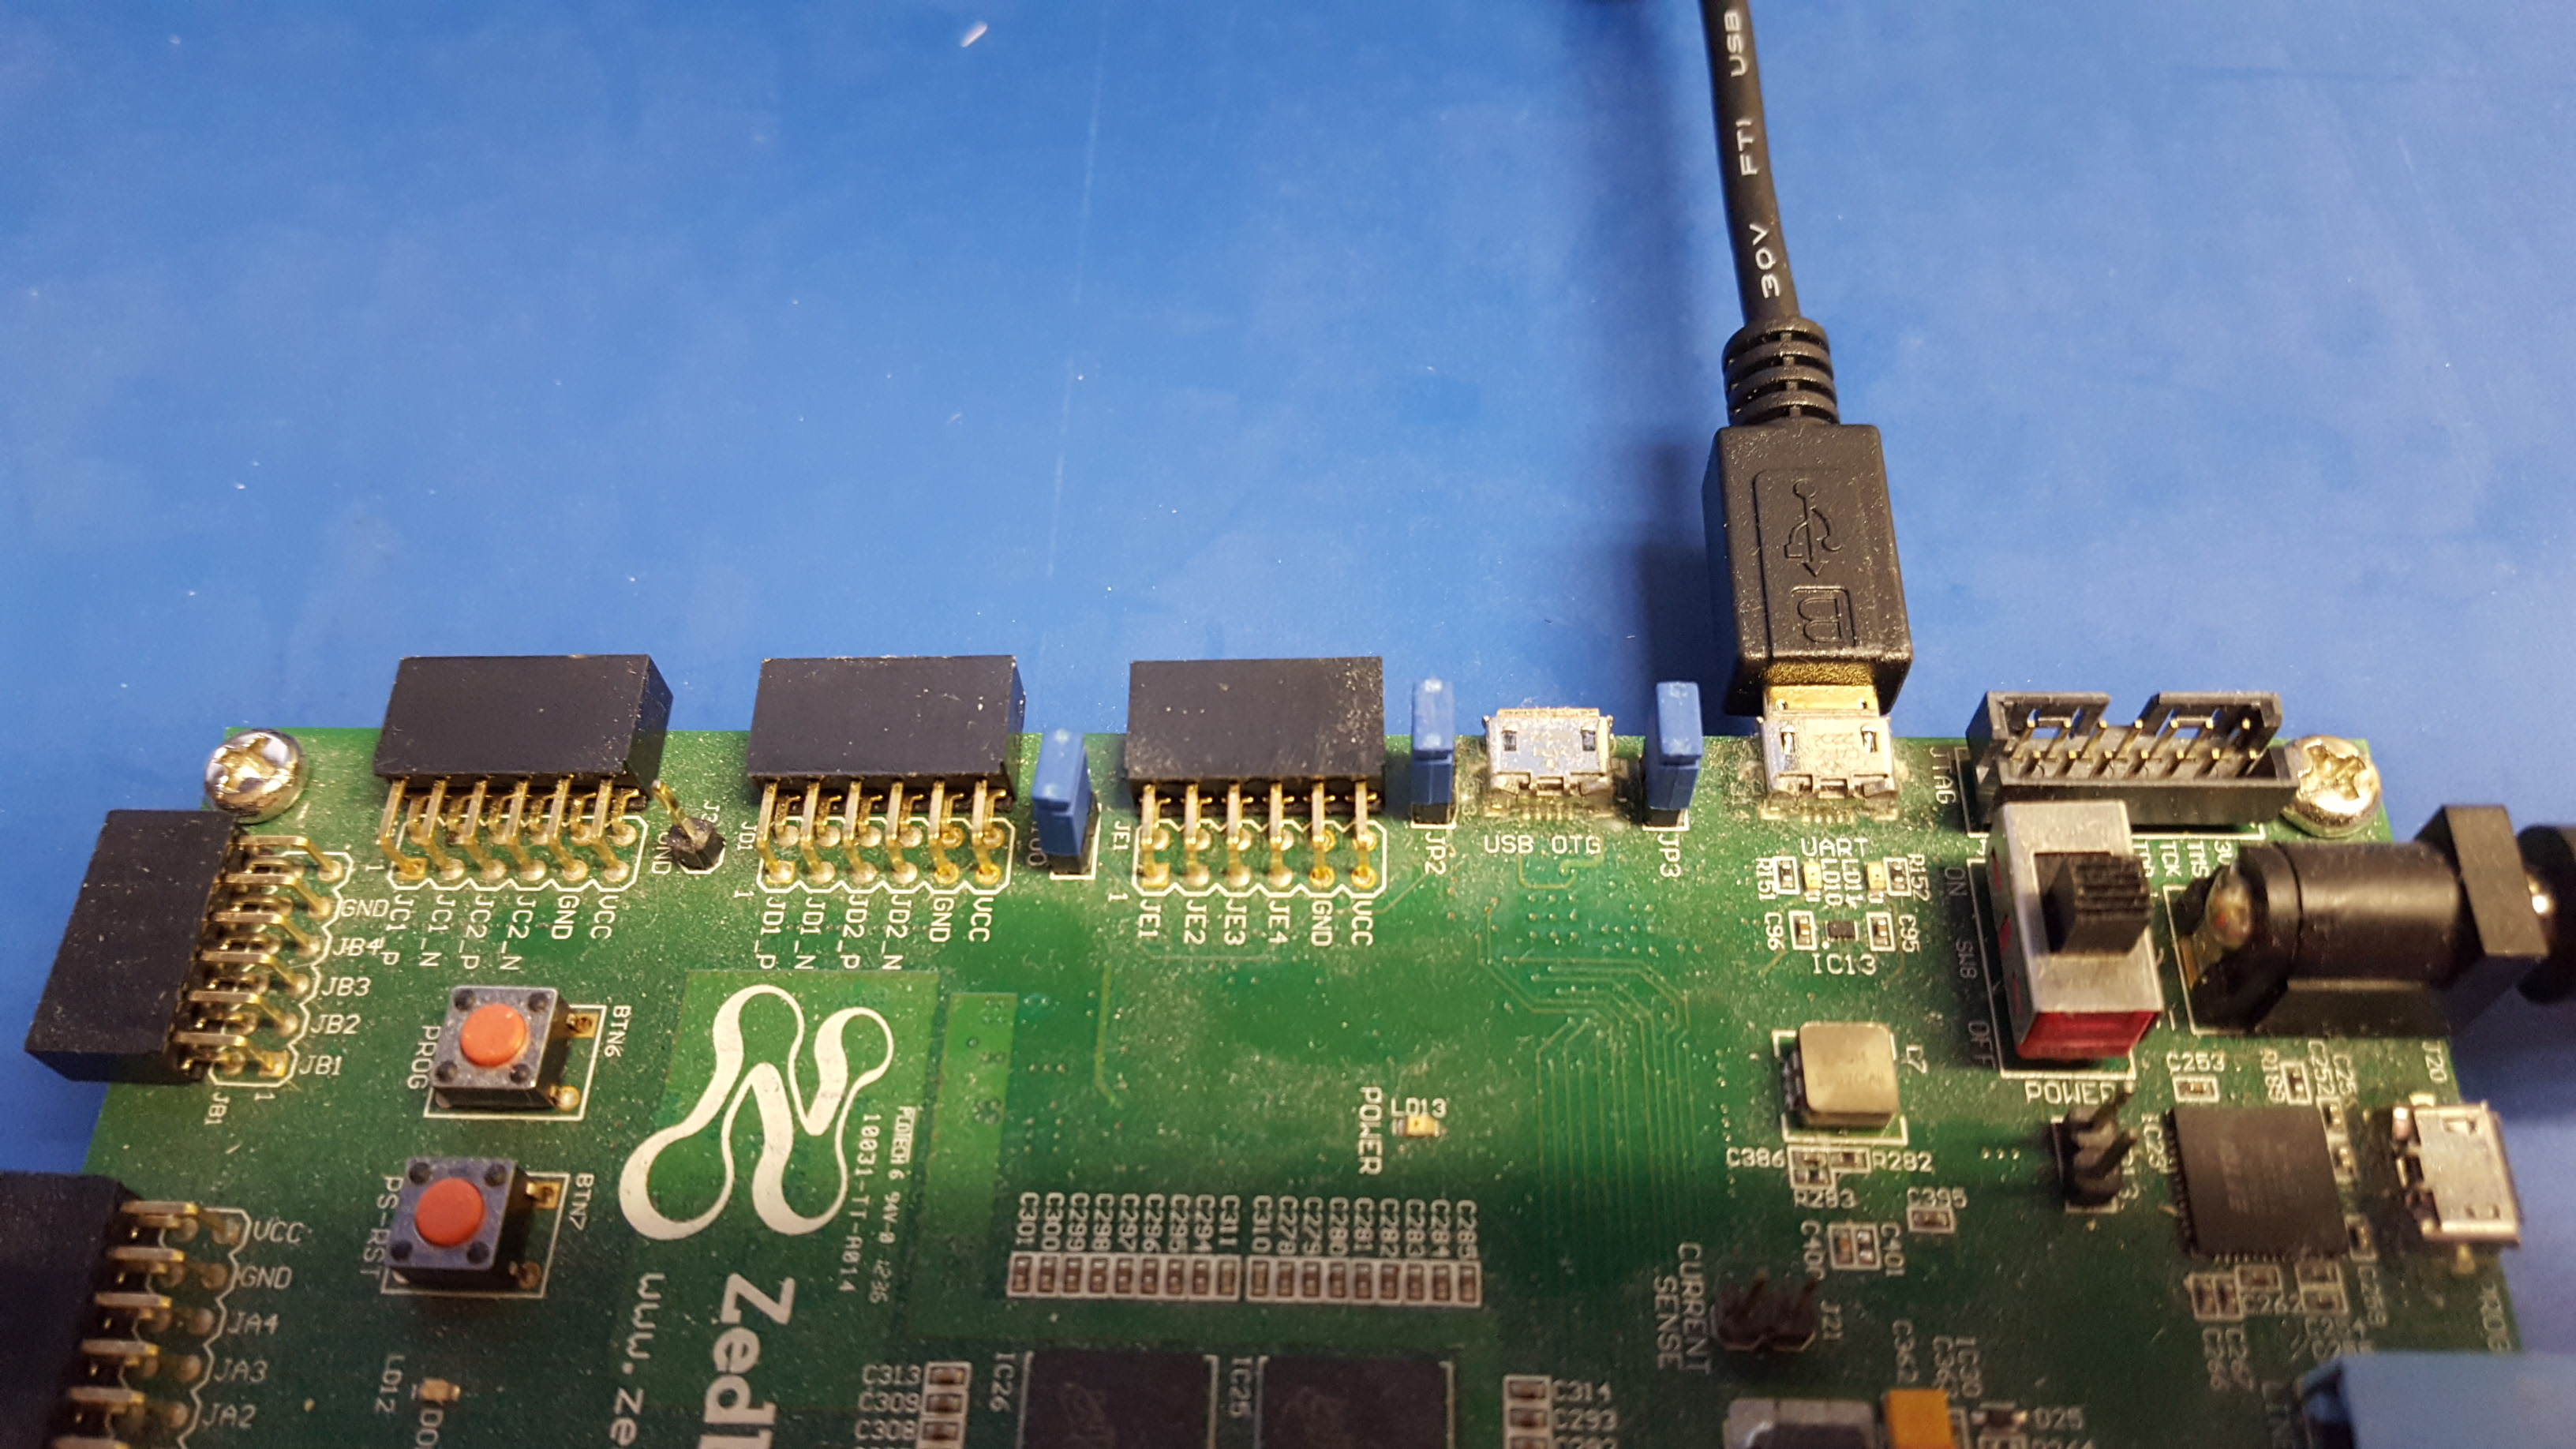
\includegraphics[scale=0.05]{zed_uart}}
	\caption{Connected Serial USB}
	\label{fig:zed_uart}
\end{figure}

Below the FMC LPC slot (bottom-side of the Zedboard), is the SD card slot which will be used throughout this guide.
\begin{figure}[H]
	\centerline{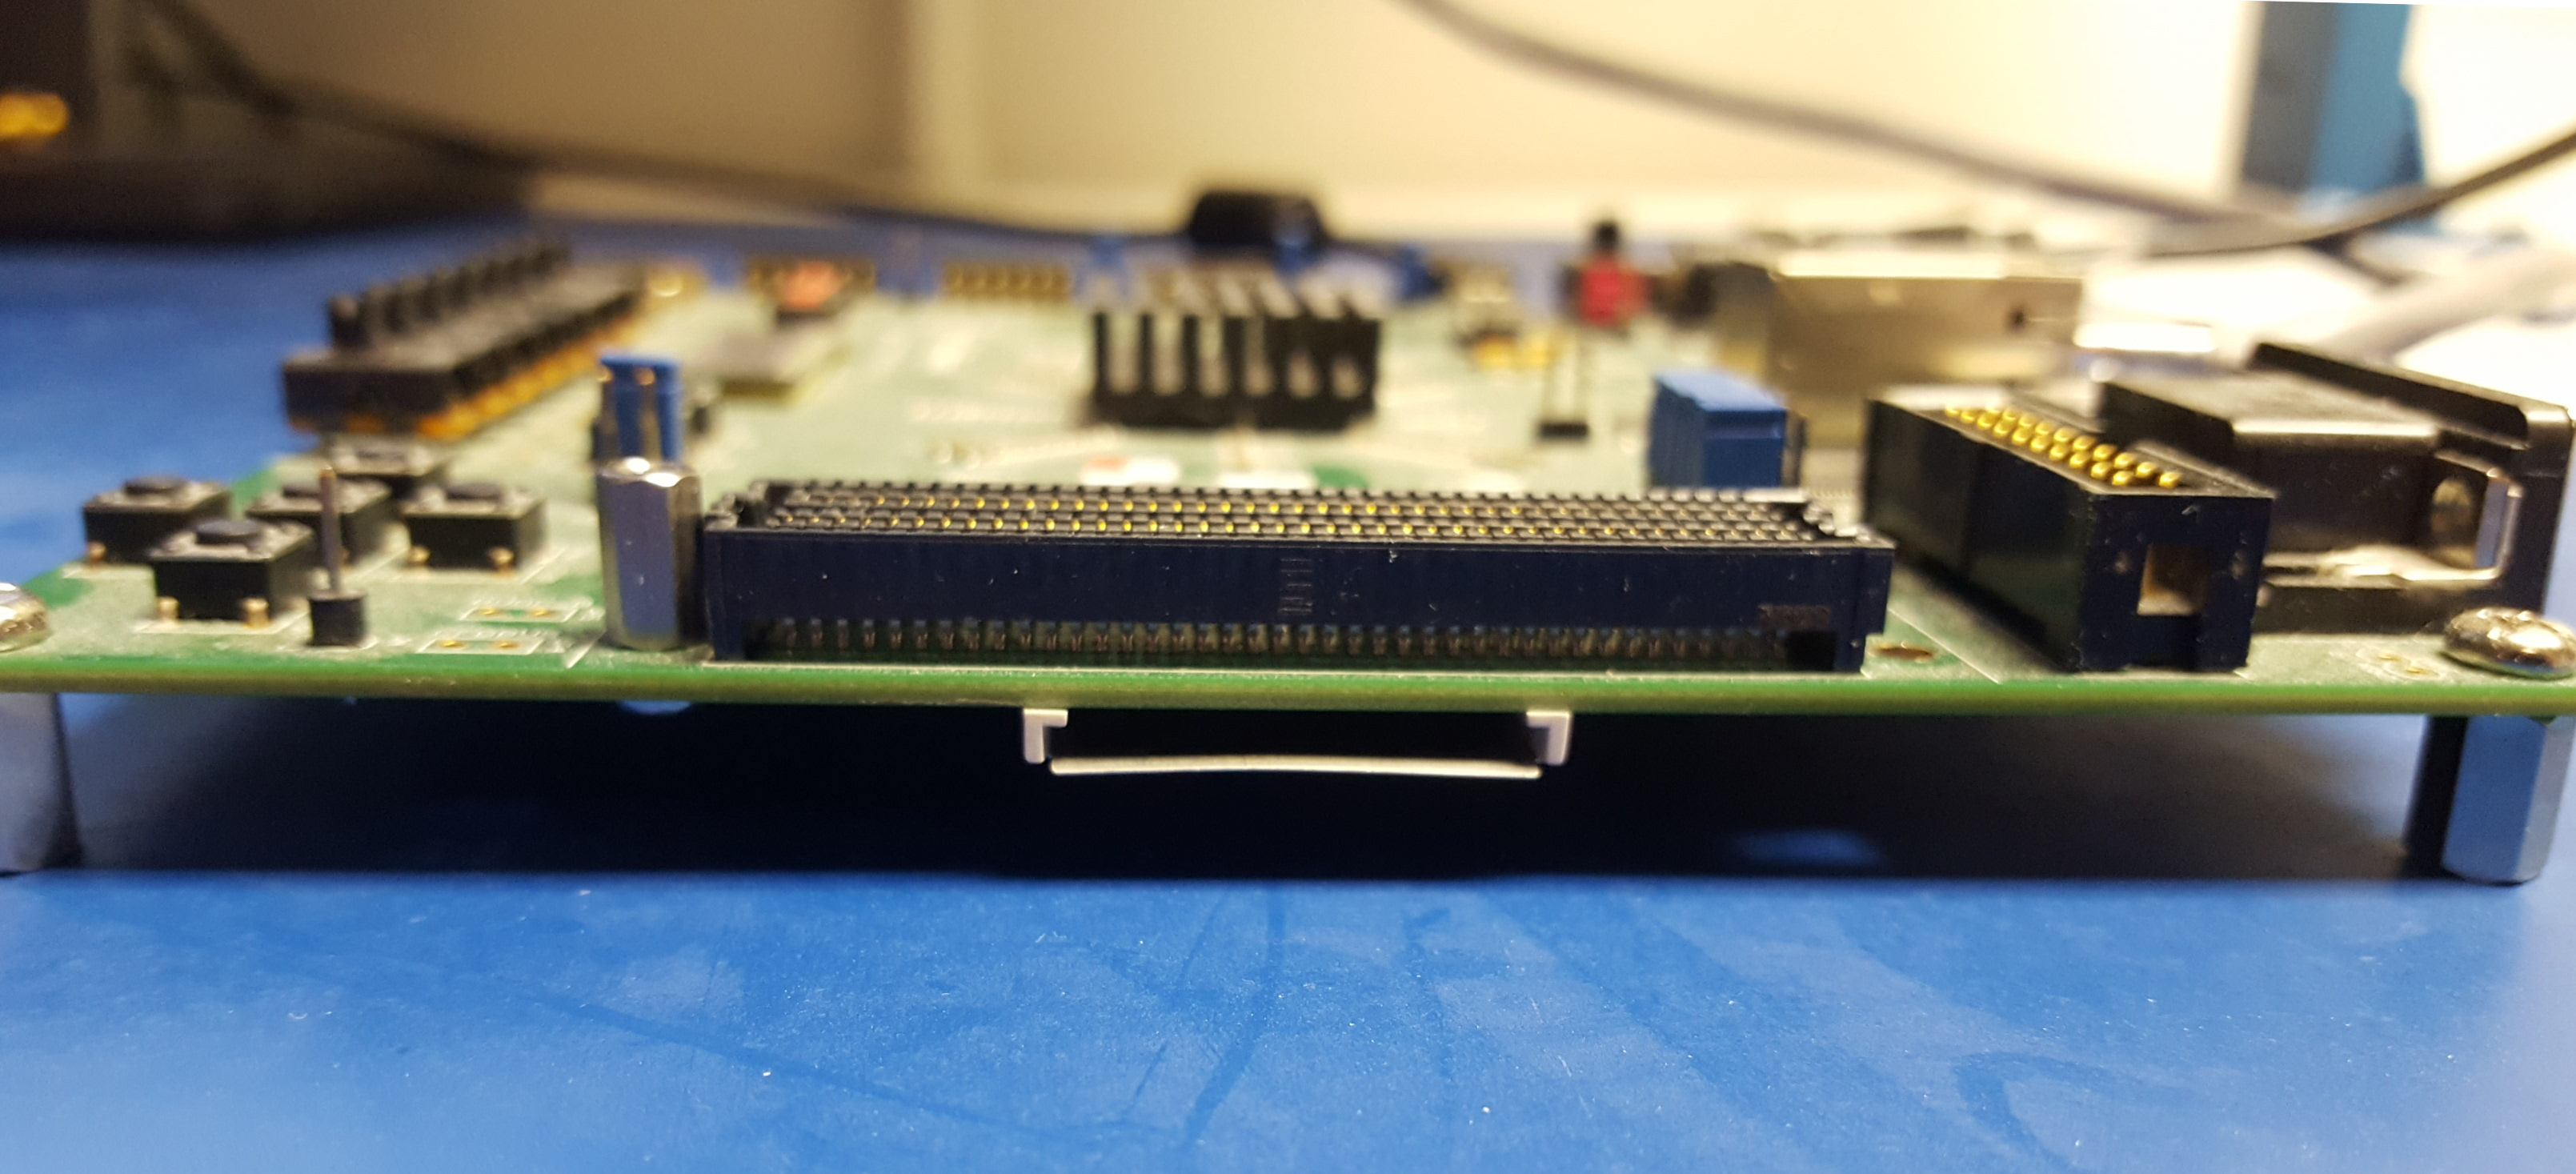
\includegraphics[scale=0.05]{zed_fmc_sd}}
	\caption{ZedBoard FMC Slot and SD card Slot}
	\label{fig:zed_fmc_sd}
\end{figure}

\item \textbf{Ethernet cable}:
An Ethernet port is available on the Zedboard and is required when the Network mode (discussed later) environment is used. The OpenCPI BSP for the ZedBoard is configured for DHCP.\medskip

\begin{figure}[H]
	\centerline{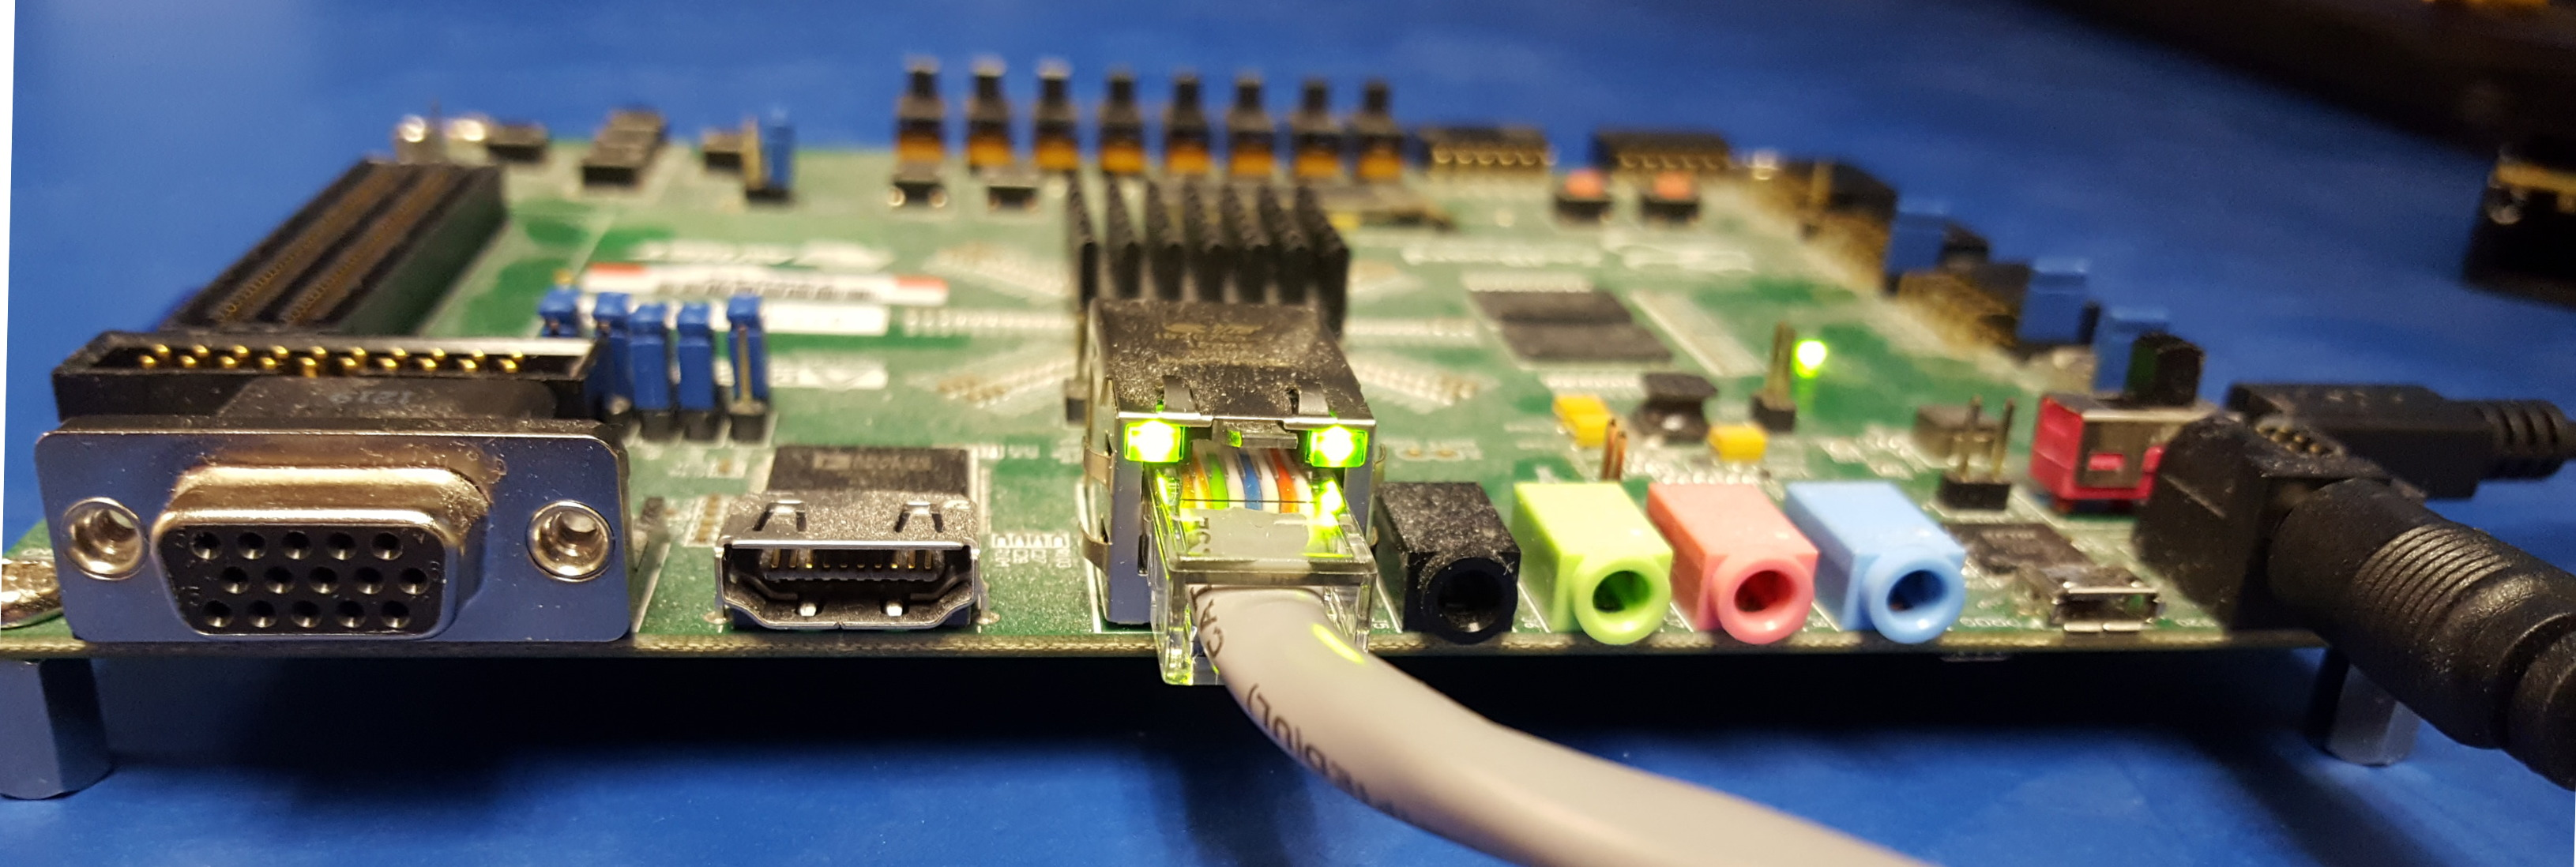
\includegraphics[scale=0.05]{zed_ether}}
	\caption{Connected Ethernet}
	\label{fig:zed_ether}
\end{figure}

\item \textbf{OpenCPI Zedboard supported daughter cards (OPTIONAL)}\\
The ZedBoard has a FMC LPC slot that is used to connect plug-in modules or daughter cards. Currently, OpenCPI supports two FMC daughter cards, which may be installed on the Zedboard:
\begin{itemize}
	\item Analog Devices FMCOMMS2
	\item Analog Devices FMCOMMS3
\end{itemize} \medskip

\item \textbf{Access to a network which supports DHCP. (Network Mode)}

\item \textbf{SD card reader}
\end{itemize}
\end{flushleft}

\section{SD Card Setup}
\label{sec:SD_Card_Setup}
The installation guide provides the procedure for creating a new SD card for OpenCPI and customizing some of files for your particular configuration.  The usual way is to make a raw copy of the manufacturer supplied card to a new card, preserving formatting and content, and then removing most original files and copying files from OpenCPI.\\ \medskip
If you need to format the SD card for this system, it should be a single FAT32 partition.

\subsection{Multiple ZedBoards on the same network}
\label{sec:Multiple ZedBoards on the same network}
If it is required that multiple ZedBoards are to be on the same network, the following change to the zynq startup scripts is required. This is necessary because by default the ZedBoards have the same MAC address from the factory. To resolve this, uncomment the following lines in the mynetsetup.sh and/or mysetup.sh scripts and modify the Ethernet address to be unique:
\begin{verbatim}
  # ifconfig eth0 down
  # ifconfig eth0 hw ether <unique MAC address> # e.g. ifconfig eth0 hw ether 00:0a:35:00:01:24
  # ifconfig eth0 up
  # udhcpc
\end{verbatim}

\pagebreak
\section{Hardware Setup}

\subsection{Establish a Serial Connection}
The installation guide provides the procedure establishing a serial console.  On ZedBoard systems the console serial port operates at 115200 baud.  The cable used is a micro-USB to USB-A cable to connect its console micro-USB port to the development host.

\subsection{Booting the ZedBoard from the SD card}
\begin{enumerate}
\item Remove power from the ZedBoard unit.
\item Ensure jumpers are configured correctly
\begin{enumerate}
\item To boot from the SD card, jumpers JP10, JP9, and JP8 need to be set to 3.3V, 3.3V, and GND respectively as shown below.
\begin{figure}[ht]
	\centerline{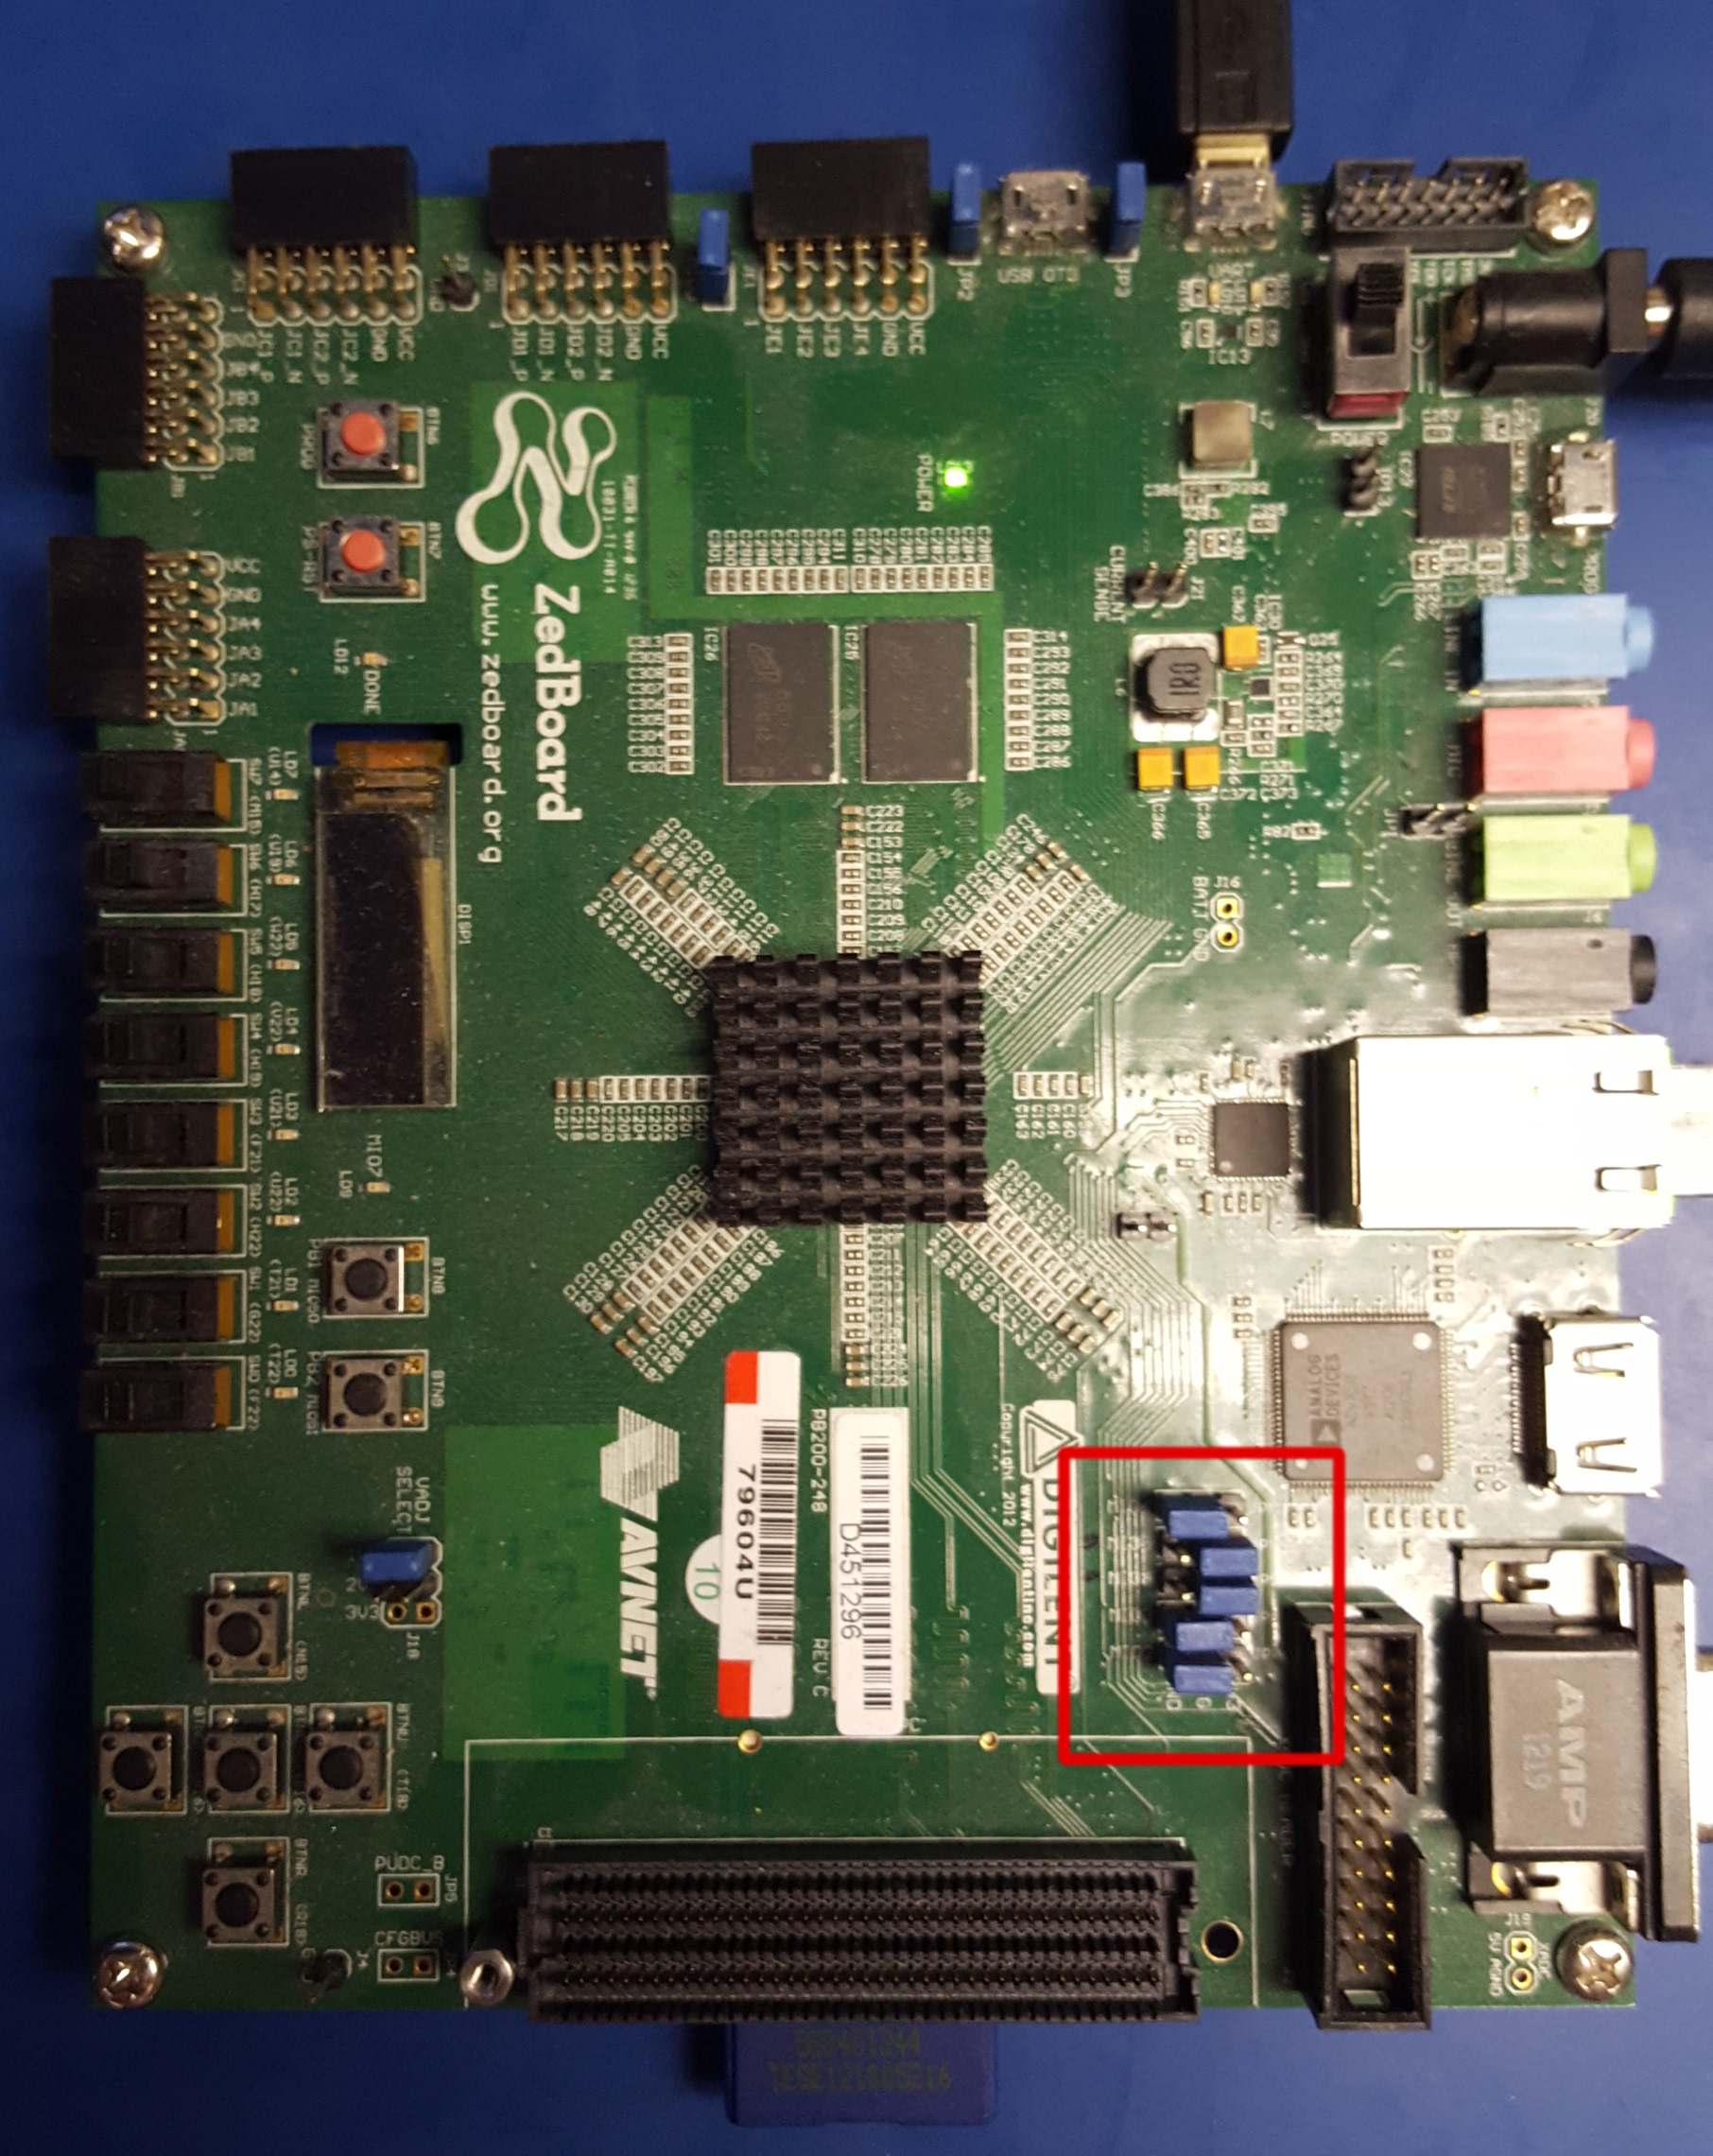
\includegraphics[scale=0.15]{zed_top}}
	\caption{Top View of the ZedBoard with J10, J9, J8 Set}
	\label{fig:zed_top}
\end{figure}
\item The only supported FMC voltage for OpenCPI Zedboard FPGA bitstreams is 2.5 V. To ensure property FMC configuration, the VADJ SELECT (J18) jumper must be set to 2V5.
\end{enumerate}
\item Insert the SD card into the SD card slot.
\item Connect a terminal to the micro-USB connector labelled 'UART' on the ZedBoard. The baud rate should be 115200 baud.
\item Start the terminal emulator on the development host (usually the \textit{screen} command) at 115200 baud.
\item Apply power to the ZedBoard with the terminal still connected.
\end{enumerate}

\section{Configuring the run-time environment on the platform}
The installation guide provides the procedure for setting up and verifying the runtime environment.
This system is initially set with  ``\textbf{root}'' for user name and password.
Typically, upon the initial power-on of the platform, the boot sequence will stop at the uboot configuration prompt. When this occurs, simply enter \textit{boot} to allow the boot sequence to continue:
\begin{verbatim}
$ zynq-uboot> boot
\end{verbatim}
\begin{flushleft}
After a successful boot to PetaLinux, login to the system, using  ``\textbf{root}`` for user name and password.

\begin{figure}[H]
	\centerline{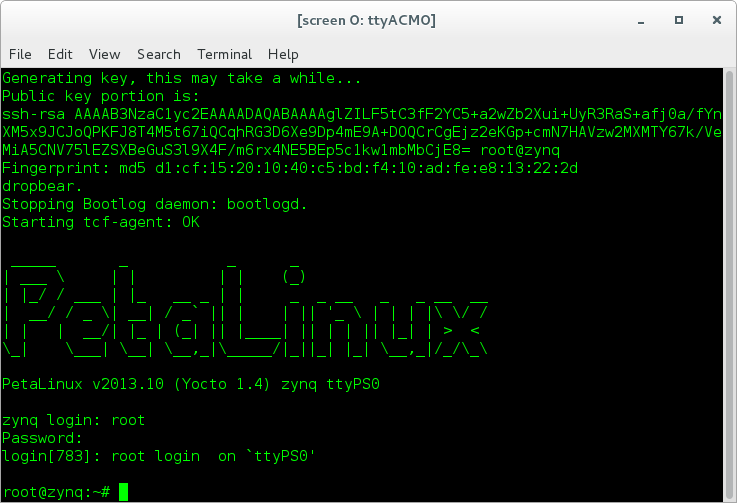
\includegraphics[scale=0.5]{zed_boot}}
	\caption{Successful Boot to PetaLinux}
	\label{fig:boot1}
\end{figure}

When a \textbf{single} Zedboard is on the network, execute the following command to enable its Ethernet interface:
\begin{verbatim}
$ ifconfig eth0 up
\end{verbatim}
When \textbf{multiple} Zedboards are on the network, the \texttt{mynetsetup.sh} script \textbf{MUST} be modified according to \ref{sec:Multiple ZedBoards on the same network} prior to proceeding to the next step, in order to prevent network collisions due to multiple Zedboards having the same MAC address.
\end{flushleft}

\section{Run an Application}
See the installation guide for running a small test application.
\pagebreak
\begin{appendices}

\section{Using ISE instead of Vivado with the ZedBoard}
\begin{flushleft}
If the user requires the use of the Xilinx ISE tools, rather than the Vivado (recommended), a different OpenCPI platform must be targeted for building bitstreams for the Zedboard. Specifically, the \textit{zed\_ise} (\textit{zynq\_ise} is the target) OpenCPI platform is built using ISE tools, where as the \textit{zed} (\textit{zynq} is the target) OpenCPI platform  is built using Vivado tools.\medskip
\end{flushleft}

% Bring in kernel message snippet
\section{Driver Notes}
\input{\snippetpath/Driver_Snippet}
%
\section{Deprecated Zipper}
\begin{flushleft}
Beginning with OpenCPI Version 1.5, support for Lime Microsystems' Zipper card is now deprecated, and the following note and figure have been removed from the main body of this Getting Started Guide:\medskip

OpenCPI has been tested on revisions C and D of the Zedboard. However, limitations have been observed for both revisions when used with the Zipper daughter-card, details are provided in Myriad-RF\_1\_Zipper\_Limitations.pdf.
\end{flushleft}

\begin{figure}[ht]
	\centerline{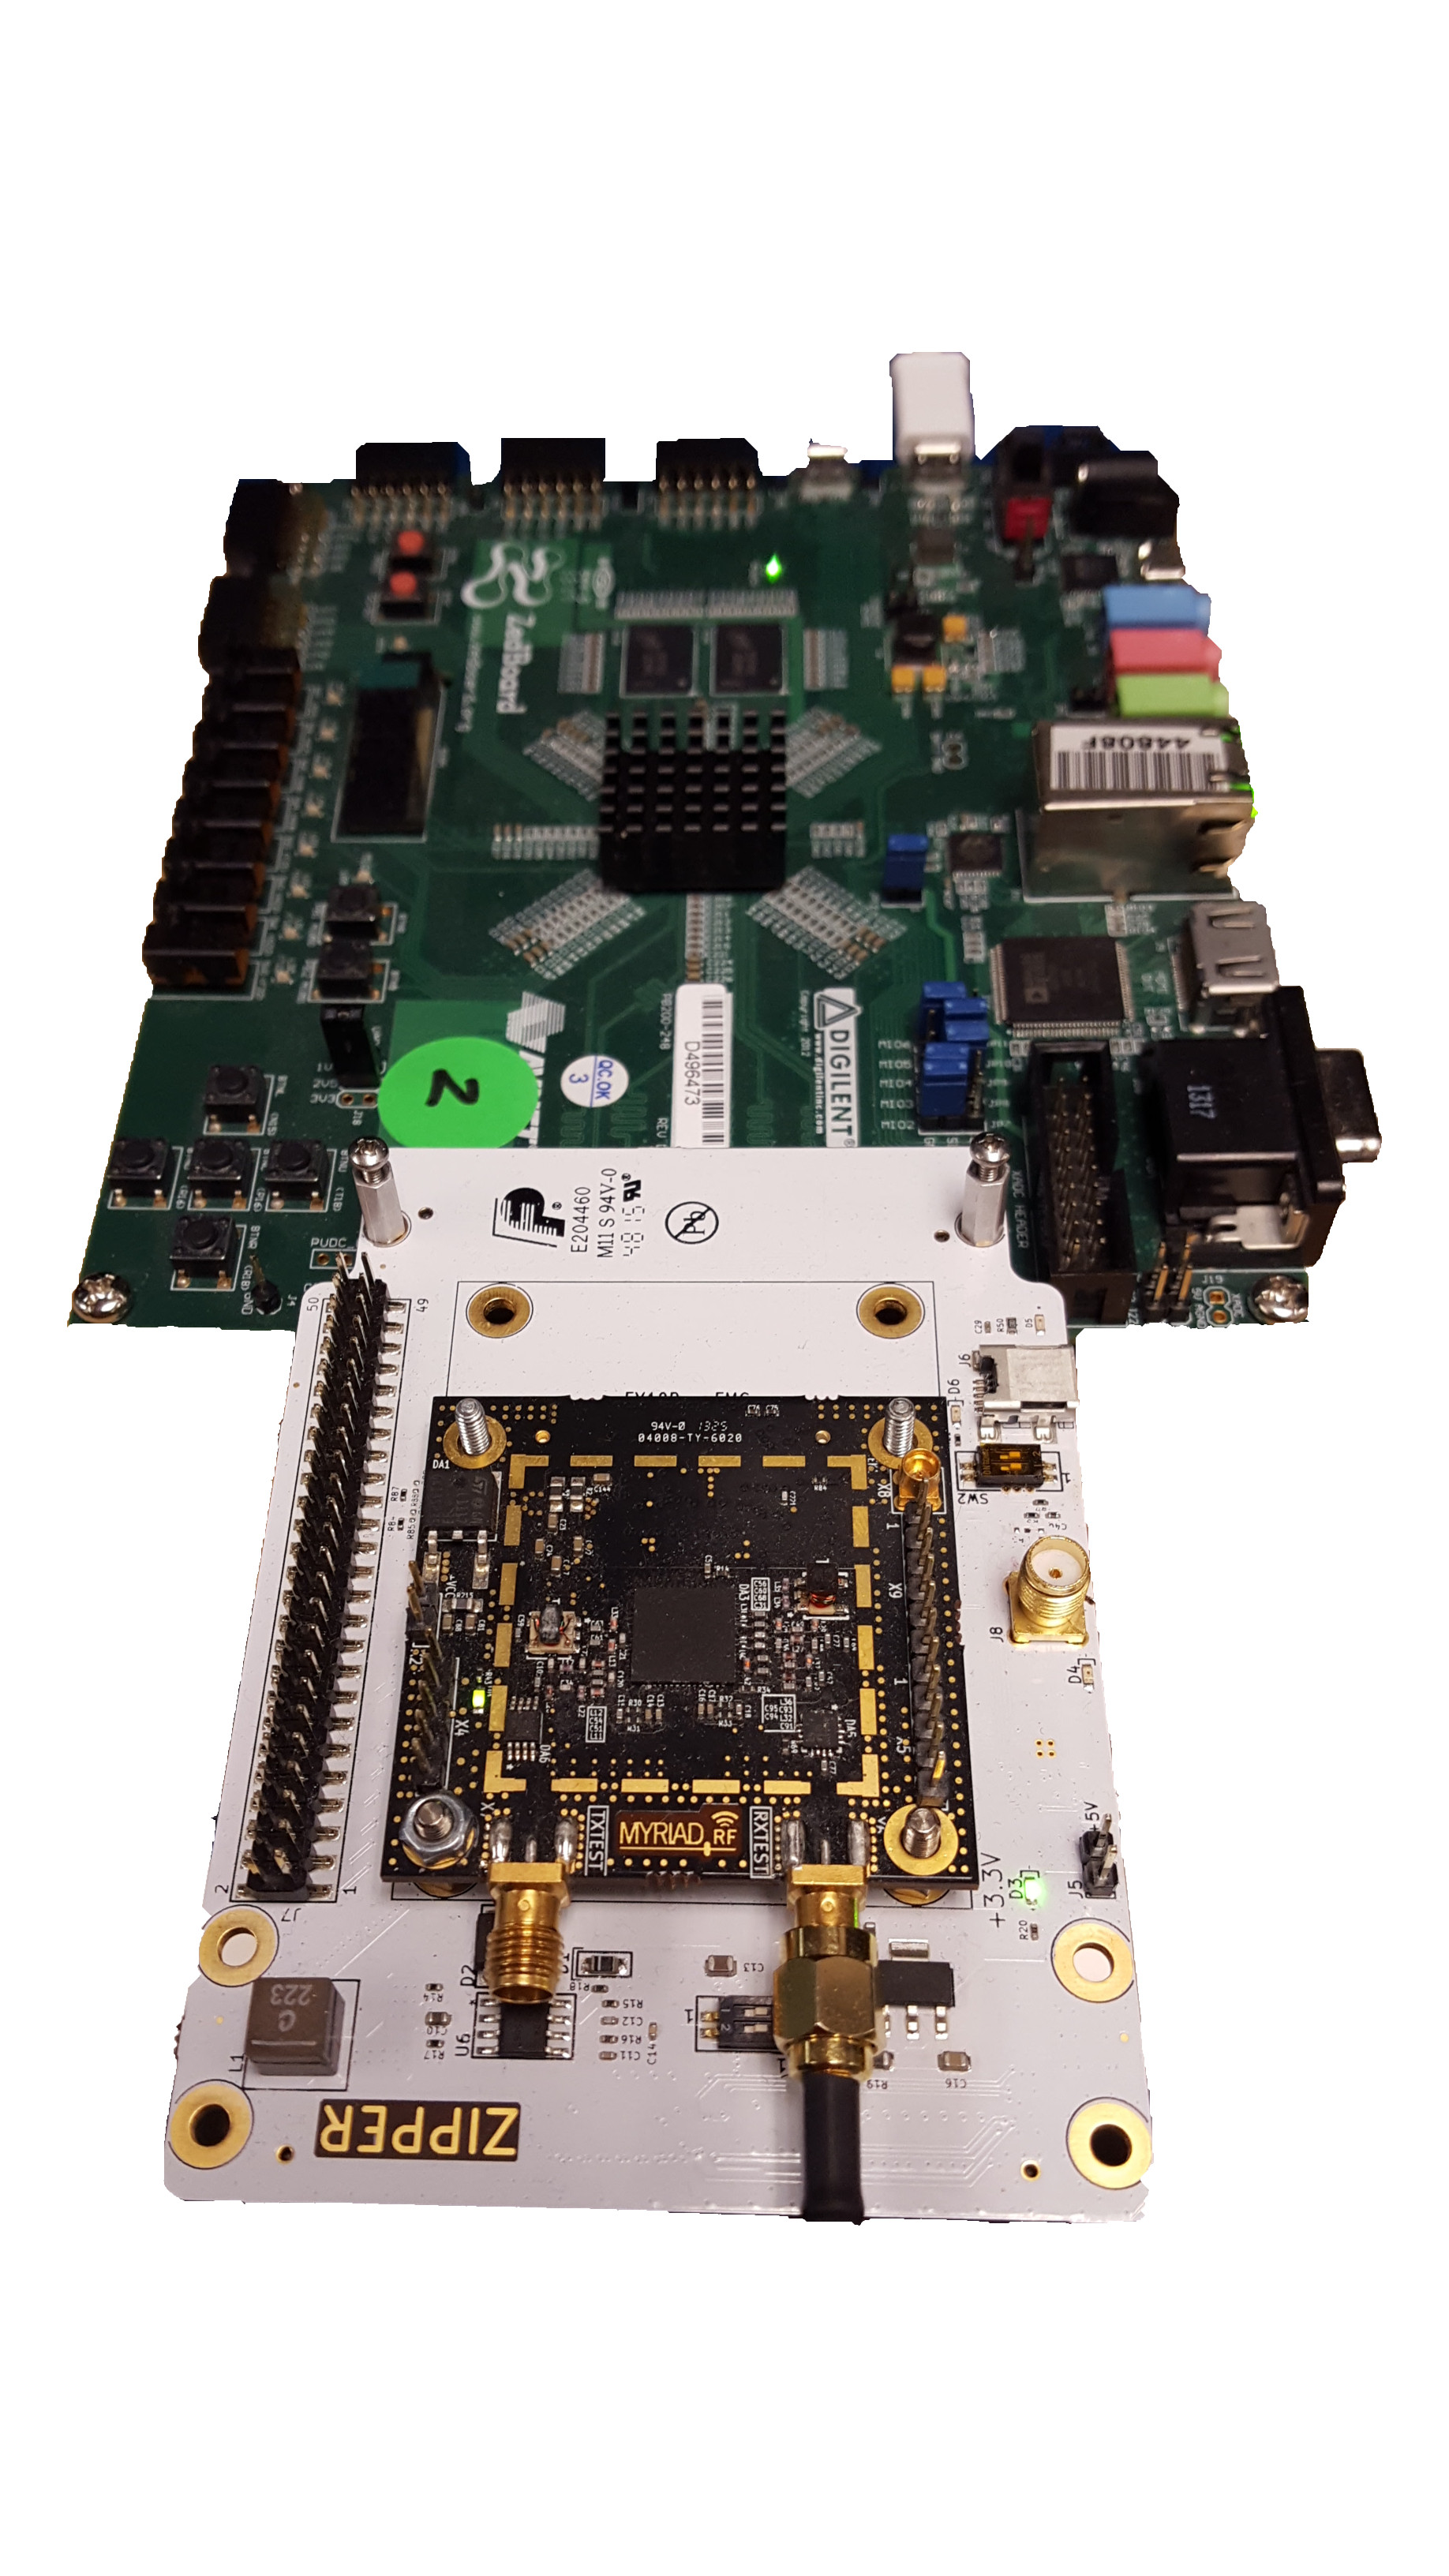
\includegraphics[scale=0.05]{zed_zipper}}
	\caption{ZedBoard With Zipper and MyriadRF-1 Connected to the FMC Slot}
	\label{fig:zed_zipper}
\end{figure}

\end{appendices}
\end{document}
